\section{Final Tables}
A graphical comparison of the background estimations to be averaged is shown in detail in appendix~\ref{app:graphical}. 
Here, the summarized results are presented in five tables: 
\begin{itemize}
\item Table~\ref{tab:OSSF1tau0} contains observed yields  and background prediction 
for each search region in a tri-lepton channel with an opposite sign same flavor lepton pair present (3$\ell$).
\item Table~\ref{tab:OSSF0tau0}  - for a channel without  an opposite sign same flavor lepton pair (no OSSF).
\item Table~\ref{tab:SStau1} - for a channel with a same sign di-lepton and a hadronically decaying tau (SS$\tau$). 
This result is fully based on Ref.~\cite{AN2012:248}.
\item Table~\ref{tab:OSOFtau1} - for a channel with an opposite sign opposite flavor di-lepton and 
a hadronically decaying tau ($e^\pm\mu^\mp\tau$). This result is provided only in Ref.~\cite{AN2012:255}.
\item Table~\ref{tab:OSSF1tau1} - for a channel with an opposite sign same flavor di-lepton and 
a hadronically decaying tau (OSSF$\tau$). This result is based on Refs.~\cite{AN2012:255}~and~\cite{AN2012:256}.
\end{itemize}

The graphical representation of the combined results is shown in Figures~\ref{fig:OSSF1tau0},~\ref{fig:OSSF0tau0},
\ref{fig:SStau1},~\ref{fig:OSOFtau1},~\ref{fig:OSSF1tau1}.

%==========================================================================================
\begin{figure}[htp]
\begin{center}
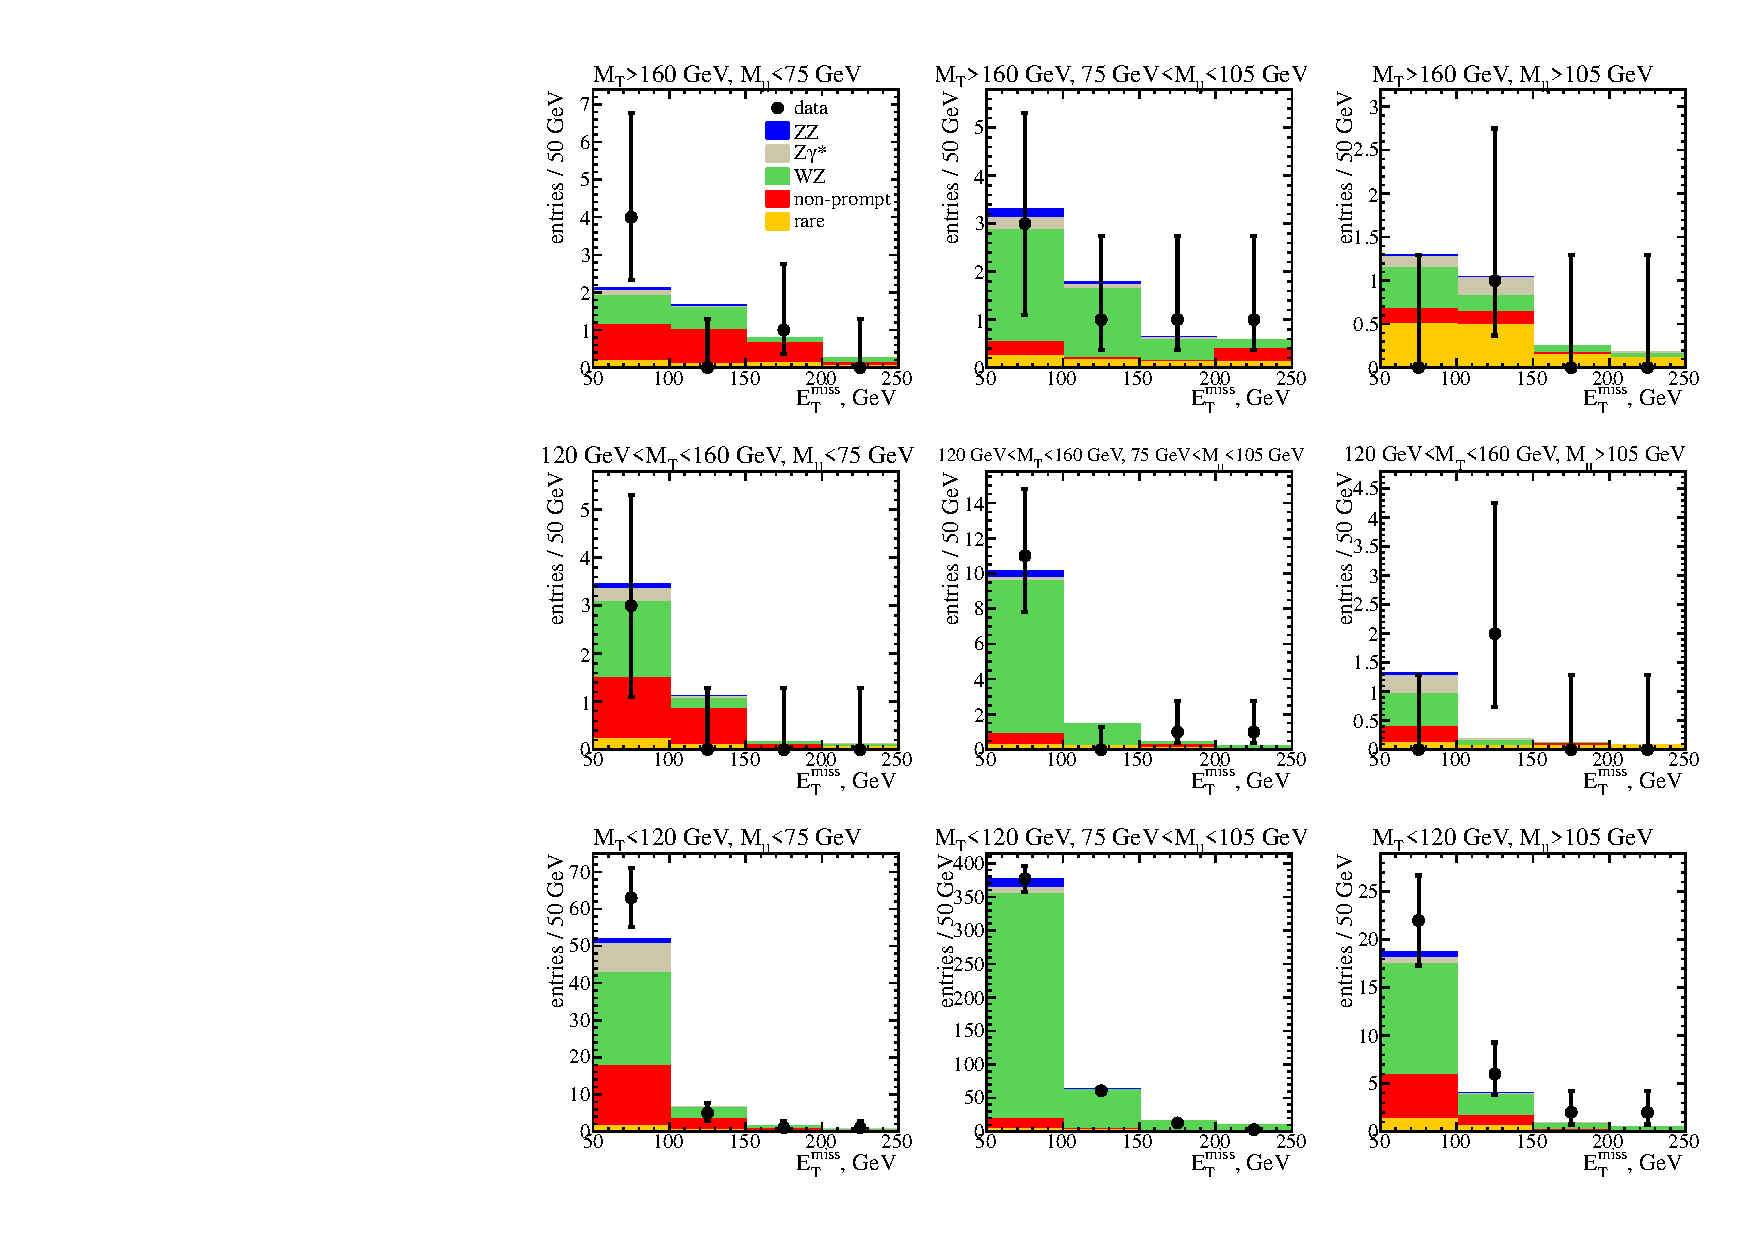
\includegraphics[width=1.0\textwidth]{plots/ossf1tau0.pdf}
\caption{Observed yields and predicted backgrounds for a tri-lepton with an opposite sign same flavor 
lepton pair present in all defined search regions.}
\label{fig:OSSF1tau0}
\end{center}
\end{figure}
%==========================================================================================
%==========================================================================================
\begin{figure}[htp]
\begin{center}
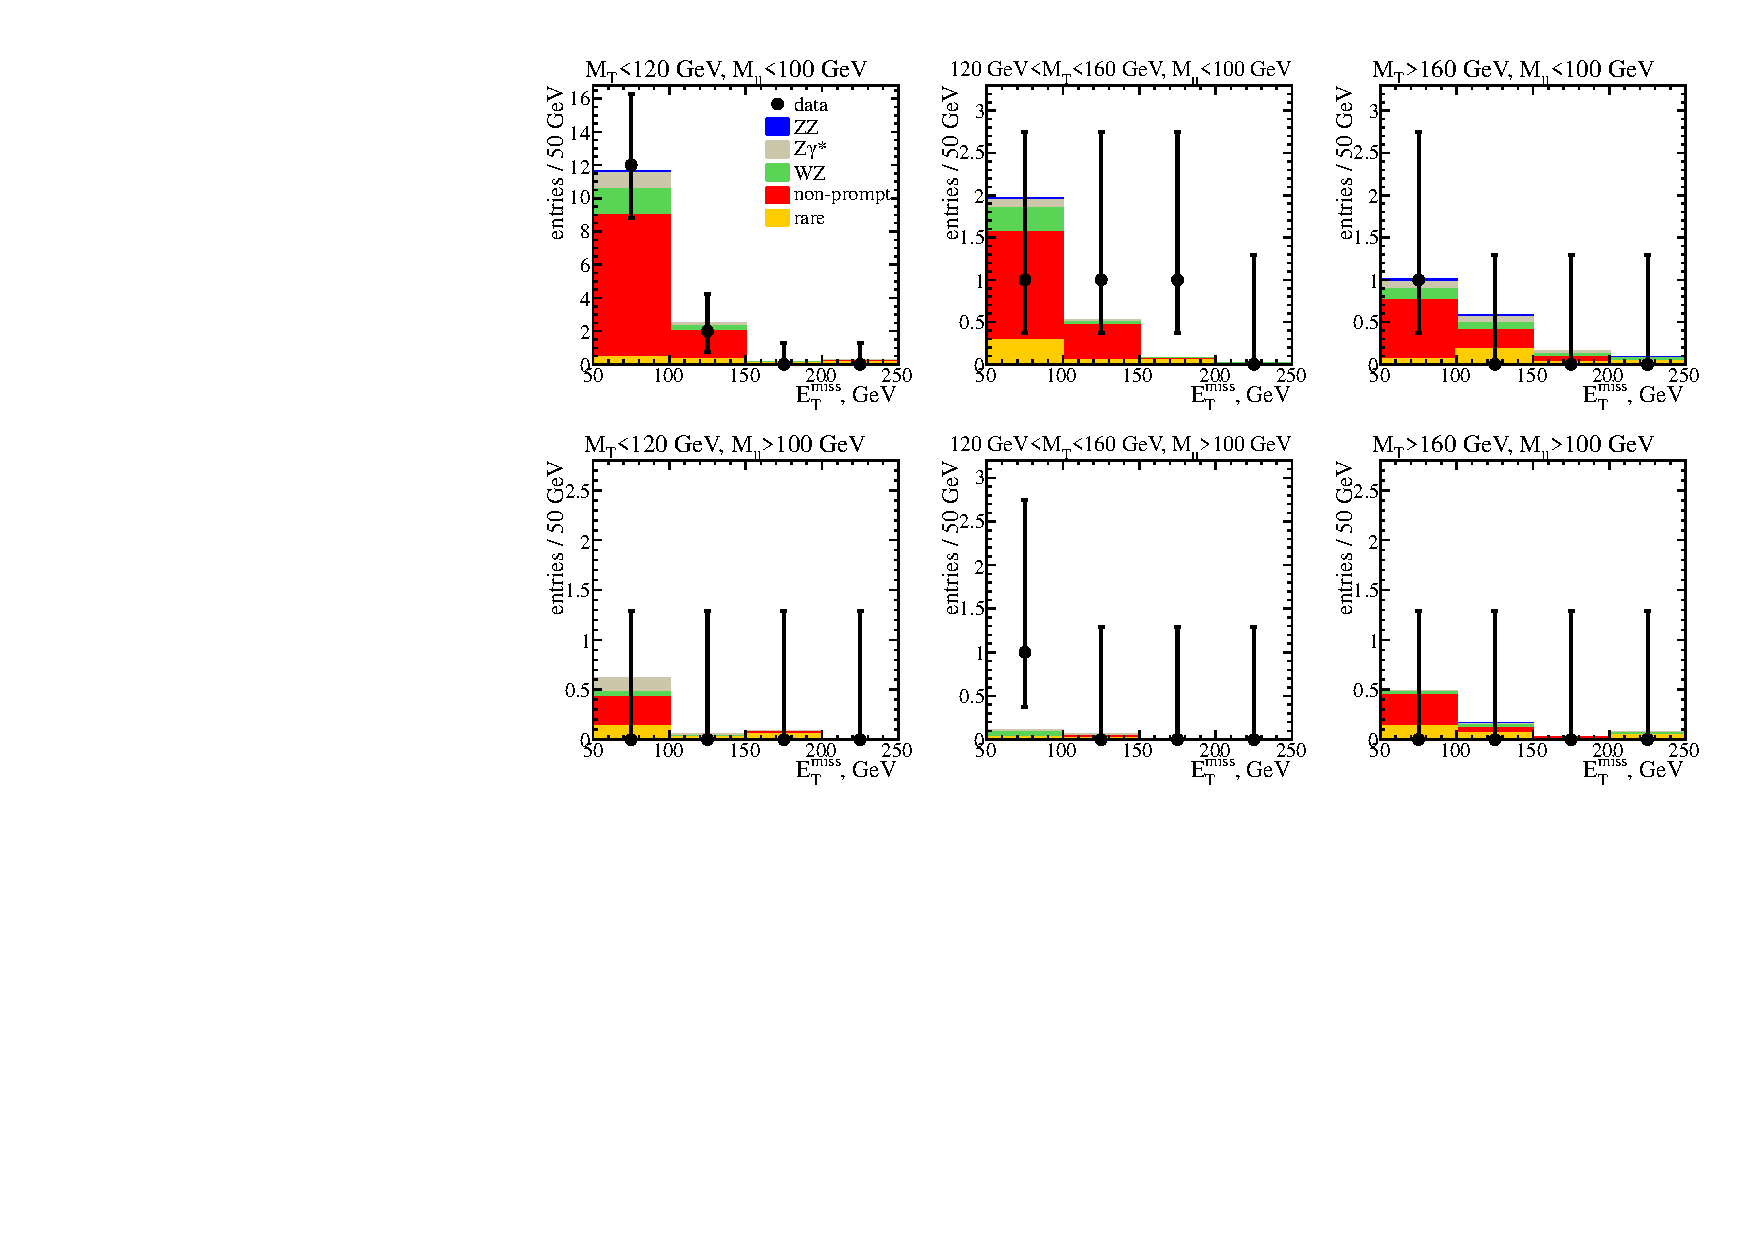
\includegraphics[width=0.95\textwidth]{plots/ossf0tau0.pdf}
\caption{Observed yields and predicted backgrounds for a tri-lepton without an opposite sign same flavor 
lepton pair present in all defined search regions.}
\label{fig:OSSF0tau0}
\end{center}
\end{figure}
%==========================================================================================
%==========================================================================================
\begin{figure}[htp]
\begin{center}
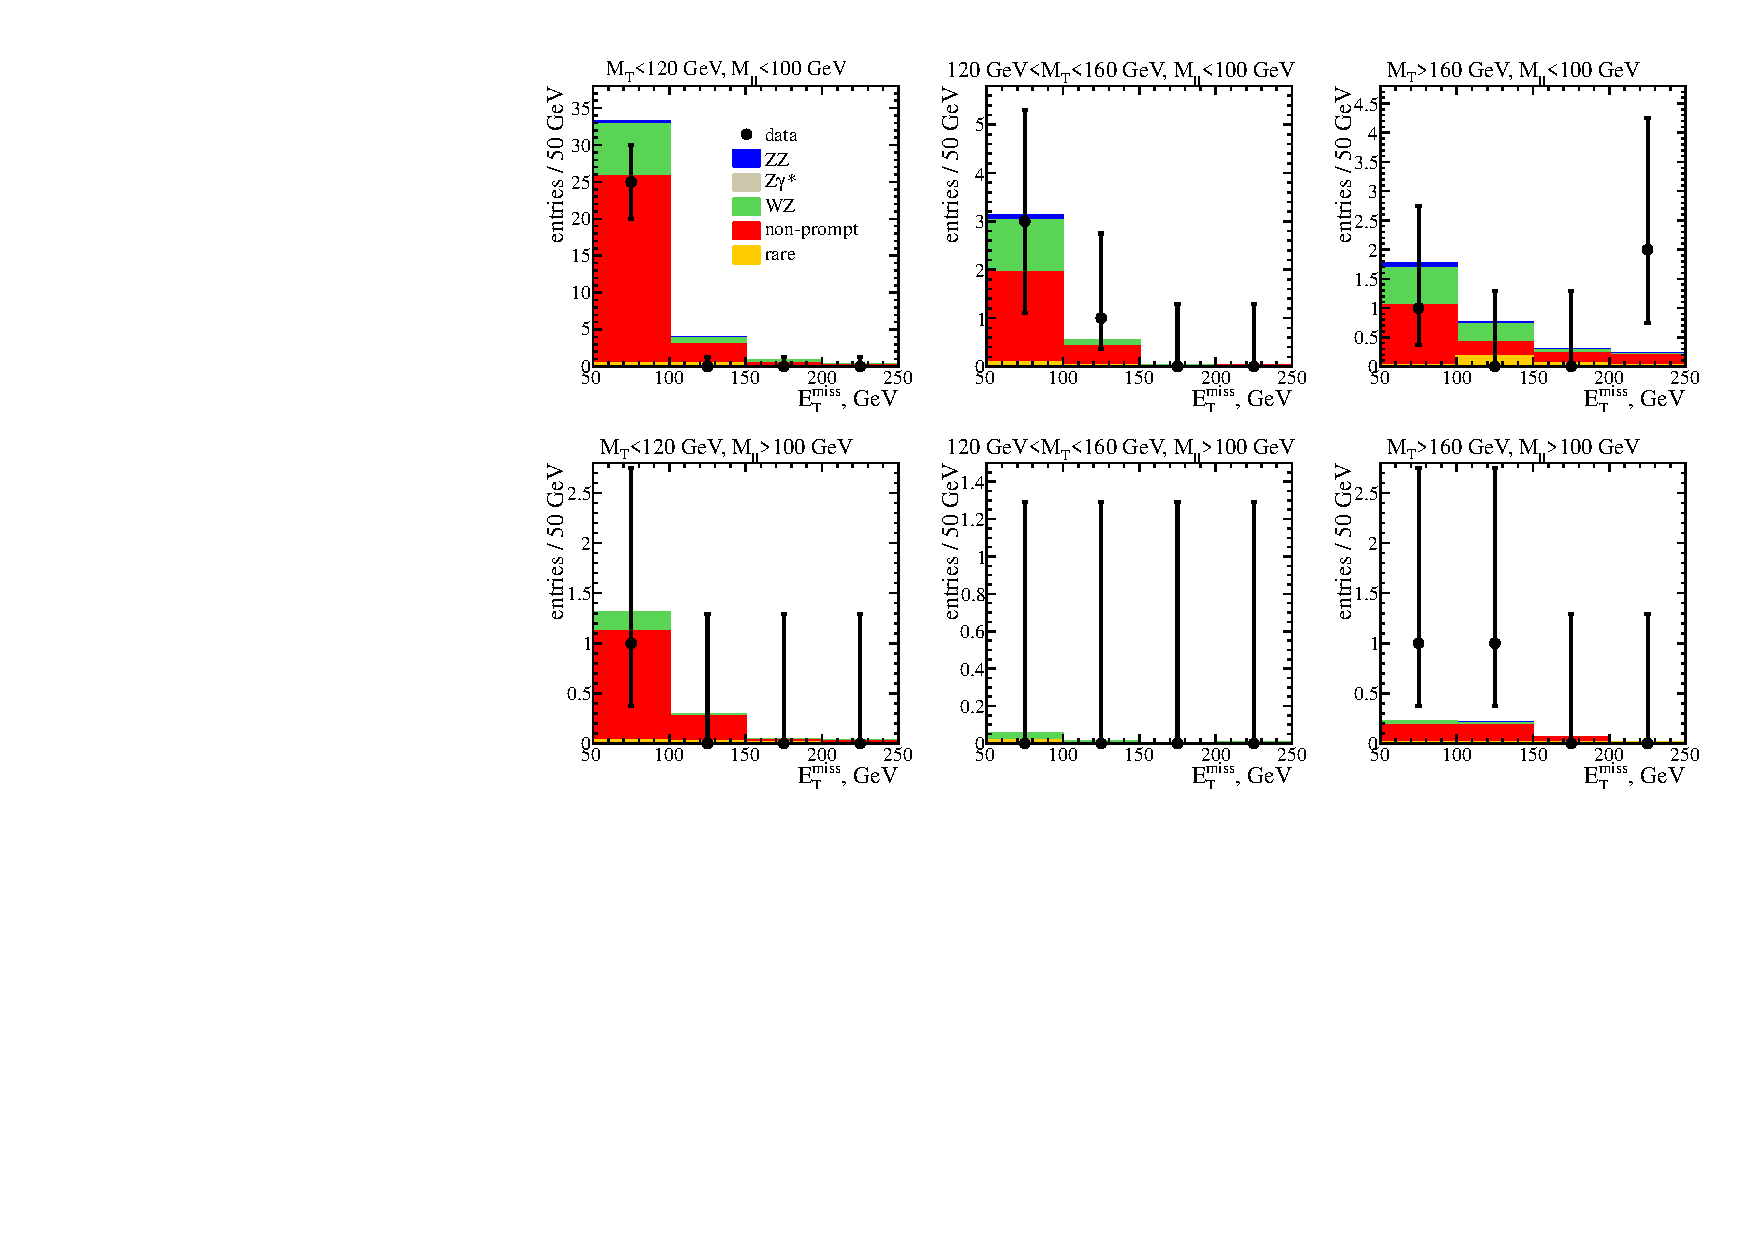
\includegraphics[width=0.95\textwidth]{plots/ossf0tau1.pdf}
\caption{Observed yields and predicted backgrounds for a tri-lepton with a same sign di-lepton 
and a hadronically decaying tau in all defined search regions.}
\label{fig:SStau1}
\end{center}
\end{figure}
%==========================================================================================
%==========================================================================================
\begin{figure}[htp]
\begin{center}
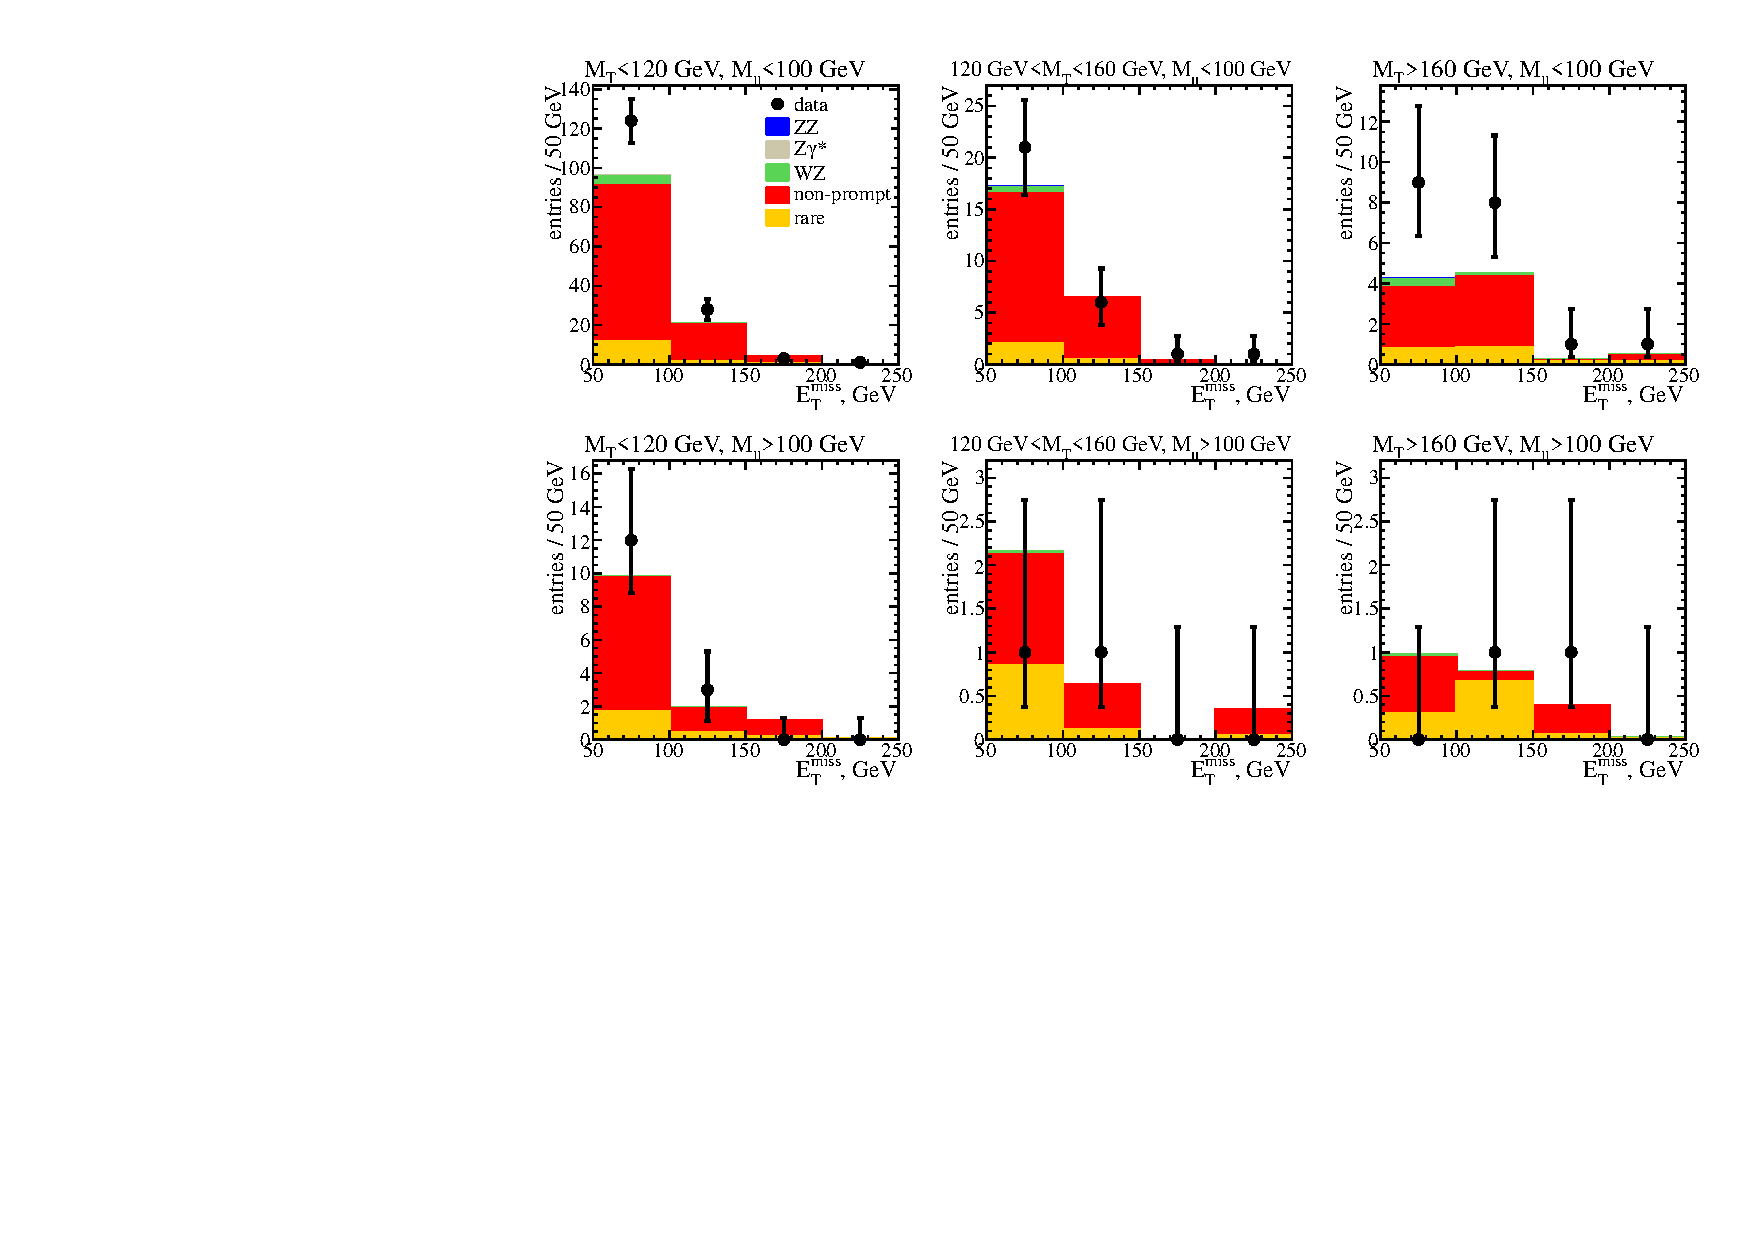
\includegraphics[width=1.0\textwidth]{plots/ossf0tau1_C2.pdf}
\caption{Observed yields and predicted backgrounds for a tri-lepton with an opposite sign opposite flavor di-lepton 
and a hadronically decaying tau in all defined search regions.}
\label{fig:OSOFtau1}
\end{center}
\end{figure}
%==========================================================================================%==========================================================================================
\begin{figure}[htp]
\begin{center}
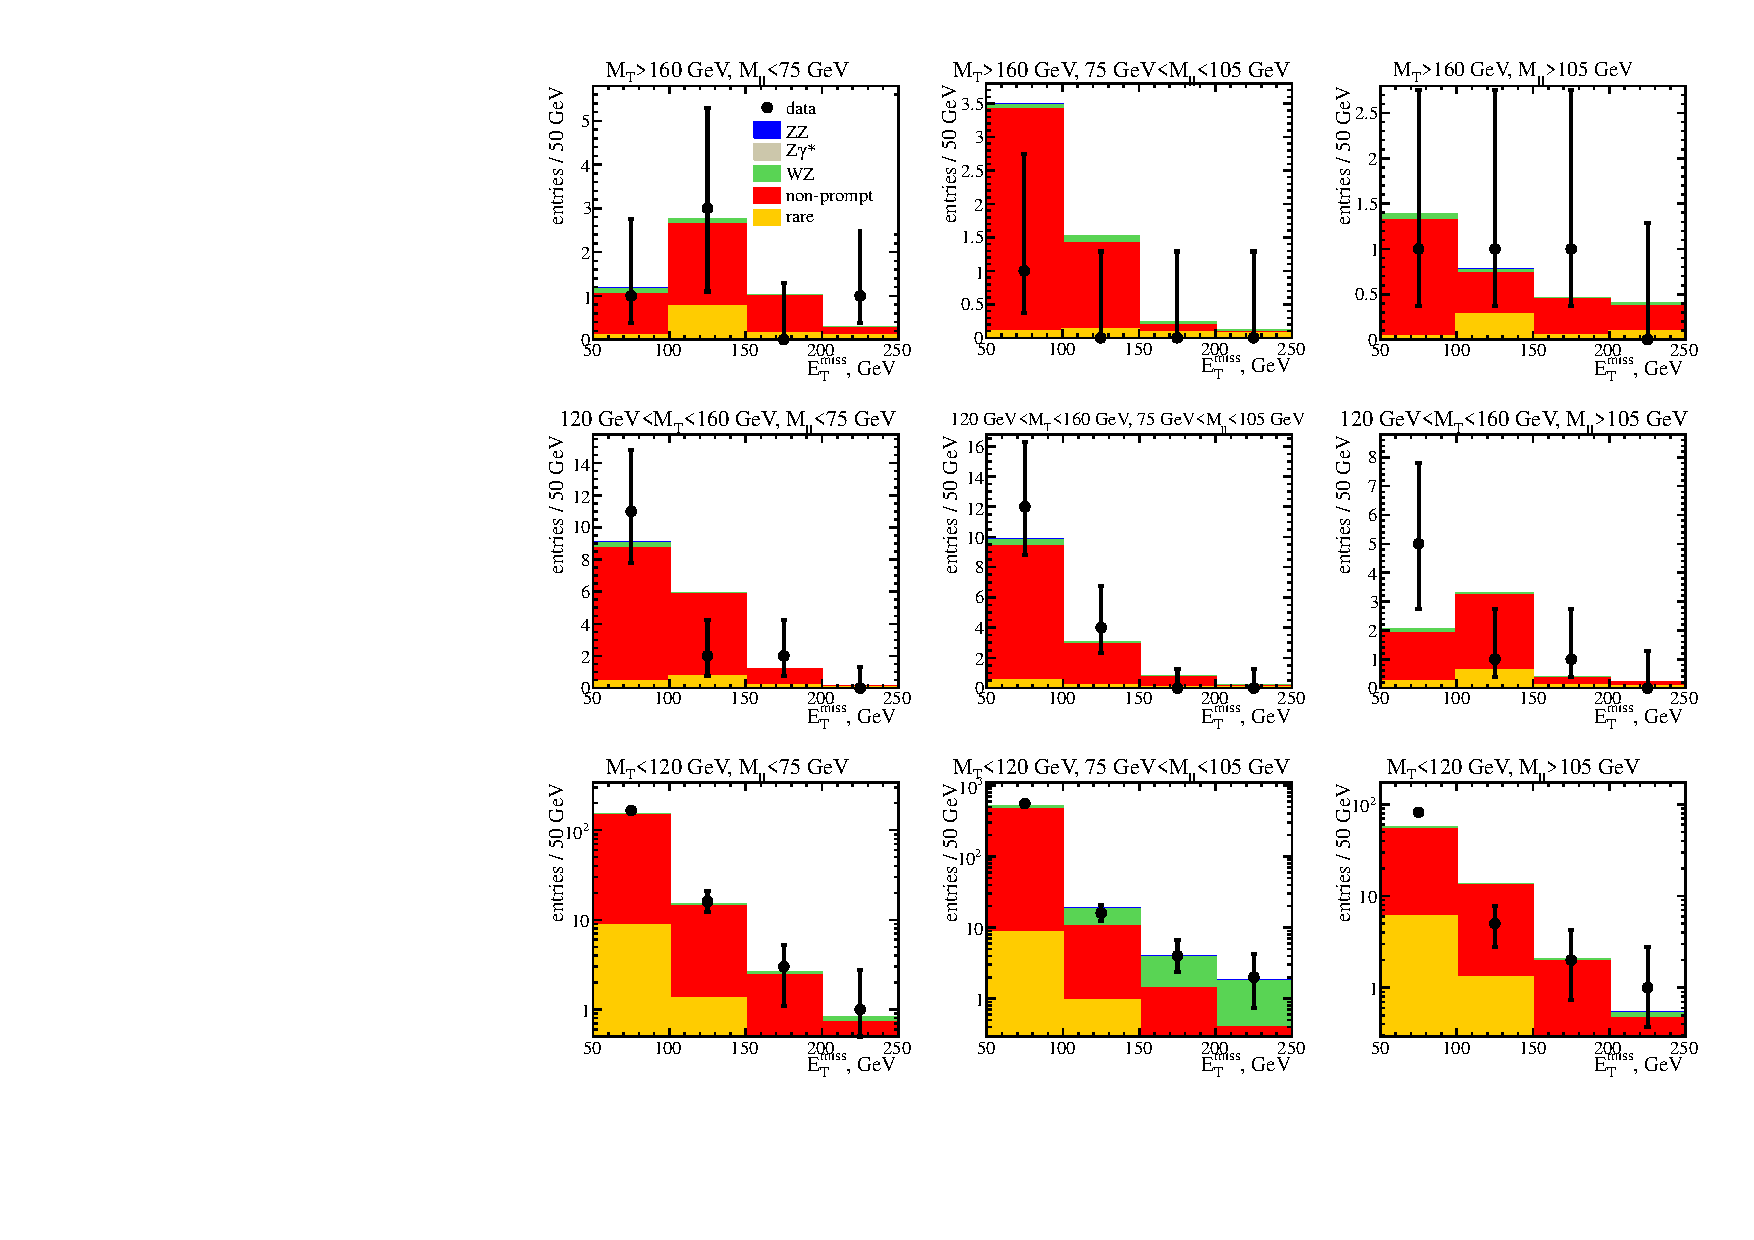
\includegraphics[width=1.0\textwidth]{plots/ossf1tau1.pdf}
\caption{Observed yields and predicted backgrounds for a tri-lepton with an opposite sign same flavor di-lepton 
and a hadronically decaying tau  in all defined search regions.}
\label{fig:OSSF1tau1}
\end{center}
\end{figure}
%==========================================================================================

\begin{landscape}
%==========================================================================================
%==========================================================================================
\begin{table}
\begin{center}
\caption{\label{tab:OSSF1tau0} The summary of the observed yields and predicted backgrounds for tri-lepton 
with opposite sign same flavor pair present. }
\begin{tabular}{| c | c c c c c c c | }\hline\hline
$\ETmiss$ (GeV) & WZ & Non-Prompt & Rare SM & Z$\gamma^*$ & ZZ & Total bkg & Observed\\\hline\hline
\multicolumn{8}{l}{$M_{\text{T}} < 120$ GeV, $M_{\ell\ell} < 75$ GeV}\\\hline\hline
50$\dots$100&26$\pm$2.7&17$\pm$3.3&1.4$\pm$0.84&8$\pm$0.36&1.3$\pm$0.028&54$\pm$4.4&63\\
100$\dots$150&3.4$\pm$0.42&3.9$\pm$0.85&0.42$\pm$0.24&0.11$\pm$0.05&0.1$\pm$0.0079&8$\pm$0.98&5\\
150$\dots$200&0.99$\pm$0.19&0.61$\pm$0.19&0.19$\pm$0.13&0.025$\pm$0.021&0.018$\pm$0.0033&1.8$\pm$0.31&1\\
200$\dots$250&0.4$\pm$0.082&0.2$\pm$0.075&0.082$\pm$0.058&0.051$\pm$0.019&0.0083$\pm$0.0018&0.74$\pm$0.13&1\\
\hline\hline
\multicolumn{8}{l}{$120~\mathrm{GeV} < M_{\text{T}} < 160~\mathrm{GeV}$, $M_{\ell\ell} < 75$ GeV}\\\hline\hline
50$\dots$100&1.6$\pm$0.22&0.97$\pm$0.38&0.22$\pm$0.14&0.27$\pm$0.065&0.1$\pm$0.008&3.2$\pm$0.47&3\\
100$\dots$150&0.24$\pm$0.038&0.61$\pm$0.3&0.091$\pm$0.067&0.051$\pm$0.028&0.015$\pm$0.0031&1$\pm$0.31&0\\
150$\dots$200&0.063$\pm$0.017&0.08$\pm$0.052&0.0046$\pm$0.0052&0$\pm$0.00059&0.00099$\pm$0.00079&0.15$\pm$0.055&0\\
200$\dots$250&0.043$\pm$0.015&0.075$\pm$0.037&0.044$\pm$0.044&0.025$\pm$0.022&0.00078$\pm$0&0.19$\pm$0.063&0\\
\hline\hline
\multicolumn{8}{l}{$M_{\text{T}} > 160$ GeV, $M_{\ell\ell} < 75$ GeV}\\\hline\hline
50$\dots$100&0.8$\pm$0.28&0.77$\pm$0.47&0.16$\pm$0.19&0.15$\pm$0.049&0.081$\pm$0.0071&2$\pm$0.58&4\\
100$\dots$150&0.6$\pm$0.21&0.75$\pm$0.54&0.096$\pm$0.11&0.025$\pm$0.019&0.045$\pm$0.0053&1.5$\pm$0.59&0\\
150$\dots$200&0.16$\pm$0.063&0.61$\pm$0.48&0.11$\pm$0.13&0$\pm$0.0059&0.011$\pm$0.0027&0.89$\pm$0.5&1\\
200$\dots$250&0.18$\pm$0.07&0.064$\pm$0.042&0.033$\pm$0.038&0$\pm$0.00024&0.0095$\pm$0.002&0.28$\pm$0.09&0\\
\hline\hline
\multicolumn{8}{l}{$M_{\text{T}} < 120$ GeV, $75~\mathrm{GeV} < M_{\ell\ell} < 105~\mathrm{GeV}$}\\\hline\hline
50$\dots$100&333$\pm$33&22.7$\pm$3.7&4.1$\pm$2.2&9.6$\pm$0.4&13.1$\pm$0.1&383$\pm$33&377\\
100$\dots$150&59$\pm$6.2&2.6$\pm$0.69&1.8$\pm$1&0.17$\pm$0.059&1.6$\pm$0.032&65$\pm$6.3&61\\
150$\dots$200&15$\pm$1.9&0.5$\pm$0.14&0.64$\pm$0.35&0.025$\pm$0.022&0.37$\pm$0.015&17$\pm$1.9&13\\
200$\dots$250&8.9$\pm$1.2&0.12$\pm$0.029&0.55$\pm$0.3&0.05$\pm$0.0011&0.15$\pm$0.0082&9.8$\pm$1.2&3\\
\hline\hline
\multicolumn{8}{l}{$120~\mathrm{GeV} < M_{\text{T}} < 160~\mathrm{GeV}$, $75~\mathrm{GeV} < M_{\ell\ell} < 105~\mathrm{GeV}$}\\\hline\hline
50$\dots$100&8.4$\pm$1.1&0.6$\pm$0.35&0.25$\pm$0.15&0.17$\pm$0.051&0.4$\pm$0.016&9.8$\pm$1.2&11\\
100$\dots$150&1.2$\pm$0.17&0.042$\pm$0.029&0.17$\pm$0.11&0$\pm$0.0064&0.032$\pm$0.0046&1.5$\pm$0.21&0\\
150$\dots$200&0.18$\pm$0.043&0.046$\pm$0.031&0.071$\pm$0.054&0$\pm$0.00033&0.0036$\pm$0.0014&0.3$\pm$0.075&1\\
200$\dots$250&0.12$\pm$0.025&0.029$\pm$0.031&0.014$\pm$0.014&0$\pm$0.00031&0.0014$\pm$0.00047&0.17$\pm$0.042&1\\
\hline\hline
\end{tabular}
\end{center}
\end{table}
%==========================================================================================
%==========================================================================================
\begin{table*}
\begin{center}
%\caption{Continuation}
\begin{tabular}{| c | c c c c c c c | }\hline\hline
$\ETmiss$ (GeV) & WZ & Non-Prompt & Rare SM & Z$\gamma^*$ & ZZ & Total bkg & Observed\\\hline\hline
\multicolumn{8}{l}{$M_{\text{T}} > 160$ GeV, $75~\mathrm{GeV} < M_{\ell\ell} < 105~\mathrm{GeV}$}\\\hline\hline
50$\dots$100&2.3$\pm$0.72&0.34$\pm$0.14&0.24$\pm$0.27&0.28$\pm$0.065&0.19$\pm$0.011&3.3$\pm$0.78&3\\
100$\dots$150&1.5$\pm$0.49&0.078$\pm$0.047&0.15$\pm$0.17&0.076$\pm$0.034&0.064$\pm$0.0065&1.9$\pm$0.53&1\\
150$\dots$200&0.48$\pm$0.17&0.015$\pm$0.016&0.12$\pm$0.14&0.051$\pm$0.027&0.015$\pm$0.0033&0.68$\pm$0.22&1\\
200$\dots$250&0.22$\pm$0.089&0.37$\pm$0.33&0.11$\pm$0.13&0$\pm$0.00012&0.007$\pm$0.0018&0.71$\pm$0.36&1\\
\hline\hline
\multicolumn{8}{l}{$M_{\text{T}} < 120$ GeV, $M_{\ell\ell} > 105$ GeV}\\\hline\hline
50$\dots$100&12$\pm$1.2&5.4$\pm$1.1&1.2$\pm$0.7&0.86$\pm$0.13&0.6$\pm$0.02&20$\pm$1.8&22\\
100$\dots$150&2.3$\pm$0.25&1.3$\pm$0.35&0.53$\pm$0.3&0.14$\pm$0.055&0.091$\pm$0.0076&4.4$\pm$0.53&6\\
150$\dots$200&0.62$\pm$0.087&0.24$\pm$0.078&0.078$\pm$0.047&0.035$\pm$0.031&0.029$\pm$0.0043&1$\pm$0.13&2\\
200$\dots$250&0.37$\pm$0.053&0.028$\pm$0.018&0.029$\pm$0.021&0$\pm$0.00062&0.014$\pm$0.0022&0.44$\pm$0.059&2\\
\hline\hline
\multicolumn{8}{l}{$120~\mathrm{GeV} < M_{\text{T}} < 160~\mathrm{GeV}$, $M_{\ell\ell} > 105$ GeV}\\\hline\hline
50$\dots$100&0.6$\pm$0.086&0.68$\pm$0.4&0.11$\pm$0.071&0.32$\pm$0.07&0.039$\pm$0.0051&1.8$\pm$0.42&0\\
100$\dots$150&0.091$\pm$0.021&0.18$\pm$0.088&0.055$\pm$0.047&0.025$\pm$0.02&0.0032$\pm$0.0014&0.35$\pm$0.1&2\\
150$\dots$200&0.033$\pm$0.01&0.052$\pm$0.033&0.055$\pm$0.049&0$\pm$0.0056&0$\pm$0&0.14$\pm$0.06&0\\
200$\dots$250&0.0019$\pm$0.0023&0.027$\pm$0.019&0.077$\pm$0.086&0$\pm$0.00021&0$\pm$0&0.11$\pm$0.088&0\\
\hline\hline
\multicolumn{8}{l}{$M_{\text{T}} > 160$ GeV, $M_{\ell\ell} > 105$ GeV}\\\hline\hline
50$\dots$100&0.46$\pm$0.16&0.38$\pm$0.19&0.5$\pm$0.66&0.16$\pm$0.055&0.025$\pm$0.0041&1.5$\pm$0.71&0\\
100$\dots$150&0.21$\pm$0.081&0.22$\pm$0.059&0.49$\pm$0.62&0.22$\pm$0.06&0.011$\pm$0.0028&1.1$\pm$0.63&1\\
150$\dots$200&0.084$\pm$0.032&0.13$\pm$0.043&0.14$\pm$0.17&0$\pm$0.012&0.0034$\pm$0.0016&0.35$\pm$0.18&0\\
200$\dots$250&0.056$\pm$0.022&0.0037$\pm$9.4e-05&0.11$\pm$0.14&0.025$\pm$0.00035&0.0036$\pm$0.00074&0.19$\pm$0.14&0\\
\hline\hline
\end{tabular}
\end{center}
\end{table*}
%==========================================================================================
%==========================================================================================
\begin{table}
\small
\begin{center}
\caption{\label{tab:OSSF0tau0} The summary of the observed yields and predicted backgrounds for tri-lepton 
without opposite sign same flavor pair present. }
\begin{tabular}{| c | c c c c c c c | }\hline\hline
$\ETmiss$ (GeV) & WZ & Non-Prompt & Rare SM & Z$\gamma^*$ & ZZ & Total bkg & Observed\\\hline\hline
\multicolumn{8}{l}{$M_{\text{T}} < 120$ GeV, $M_{\ell\ell} < 100$ GeV}\\\hline\hline
50$\dots$100&1.6$\pm$0.16&8.7$\pm$2&0.44$\pm$0.26&1.1$\pm$0.11&0.11$\pm$0.0082&12$\pm$2&12\\
100$\dots$150&0.32$\pm$0.053&2$\pm$0.47&0.29$\pm$0.18&0.24$\pm$0.048&0.01$\pm$0.0026&2.8$\pm$0.51&2\\
150$\dots$200&0.085$\pm$0.026&0.35$\pm$0.12&0.062$\pm$0.05&0.029$\pm$0.018&0.0023$\pm$0.0012&0.53$\pm$0.13&0\\
200$\dots$250&0.029$\pm$0.0081&0.15$\pm$0.062&0.13$\pm$0.14&0.038$\pm$0.018&0.00099$\pm$0.0008&0.35$\pm$0.15&0\\
\hline\hline
\multicolumn{8}{l}{$120~\mathrm{GeV} < M_{\text{T}} < 160~\mathrm{GeV}$, $M_{\ell\ell} < 100$ GeV}\\\hline\hline
50$\dots$100&0.29$\pm$0.042&1.4$\pm$0.47&0.28$\pm$0.22&0.12$\pm$0.035&0.029$\pm$0.0041&2.2$\pm$0.52&1\\
100$\dots$150&0.029$\pm$0.011&0.4$\pm$0.13&0.051$\pm$0.036&0.038$\pm$0.018&0.0042$\pm$0.0016&0.52$\pm$0.14&1\\
150$\dots$200&0.019$\pm$0.0084&0.072$\pm$0.028&0.047$\pm$0.046&0$\pm$0.0061&0$\pm$0&0.14$\pm$0.055&1\\
200$\dots$250&0.003$\pm$0.0038&0.02$\pm$0.0023&0.0068$\pm$0.0062&0$\pm$0&0$\pm$0&0.029$\pm$0.0076&0\\
\hline\hline
\multicolumn{8}{l}{$M_{\text{T}} > 160$ GeV, $M_{\ell\ell} < 100$ GeV}\\\hline\hline
50$\dots$100&0.14$\pm$0.051&0.84$\pm$0.31&0.058$\pm$0.068&0.11$\pm$0.031&0.026$\pm$0.0041&1.2$\pm$0.32&1\\
100$\dots$150&0.11$\pm$0.044&0.83$\pm$0.35&0.18$\pm$0.23&0.093$\pm$0.029&0.028$\pm$0.0044&1.2$\pm$0.42&0\\
150$\dots$200&0.033$\pm$0.014&0.1$\pm$0.059&0.022$\pm$0.026&0.029$\pm$0.014&0.0037$\pm$0.0014&0.19$\pm$0.068&0\\
200$\dots$250&0.04$\pm$0.019&0.038$\pm$0.018&0.039$\pm$0.047&0$\pm$0.00017&0.0043$\pm$0.0014&0.12$\pm$0.054&0\\
\hline\hline
\multicolumn{8}{l}{$M_{\text{T}} < 120$ GeV, $M_{\ell\ell} > 100$ GeV}\\\hline\hline
50$\dots$100&0.041$\pm$0.012&0.5$\pm$0.15&0.14$\pm$0.086&0.21$\pm$0.042&0.0021$\pm$0.0012&0.89$\pm$0.18&0\\
100$\dots$150&0.0064$\pm$0.0037&0.14$\pm$0.031&0.025$\pm$0.019&0.038$\pm$0.019&0$\pm$0&0.21$\pm$0.041&0\\
150$\dots$200&0$\pm$0&0.062$\pm$0.028&0.056$\pm$0.049&0.013$\pm$0.01&0.00011$\pm$0.00011&0.13$\pm$0.057&0\\
200$\dots$250&0$\pm$0&0.02$\pm$0.012&0.00021$\pm$0.00017&0$\pm$0.0052&0$\pm$0&0.02$\pm$0.014&0\\
\hline\hline
\multicolumn{8}{l}{$120~\mathrm{GeV} < M_{\text{T}} < 160~\mathrm{GeV}$, $M_{\ell\ell} > 100$ GeV}\\\hline\hline
50$\dots$100&0.057$\pm$0.013&0.002$\pm$0.0014&0.023$\pm$0.019&0.025$\pm$0.014&0.00088$\pm$0.00064&0.11$\pm$0.027&1\\
100$\dots$150&0.0037$\pm$0.0036&0.024$\pm$0.022&0.014$\pm$0.014&0.025$\pm$0.014&0$\pm$0&0.067$\pm$0.03&0\\
150$\dots$200&0$\pm$0&0$\pm$0&0.00021$\pm$0.00018&0$\pm$4.1e-05&0$\pm$0&0.00021$\pm$0.00019&0\\
200$\dots$250&0$\pm$0&0$\pm$1.8e-05&0.004$\pm$0.0046&0$\pm$3.4e-05&0$\pm$0&0.004$\pm$0.0046&0\\
\hline\hline
\multicolumn{8}{l}{$M_{\text{T}} > 160$ GeV, $M_{\ell\ell} > 100$ GeV}\\\hline\hline
50$\dots$100&0.022$\pm$0.011&0.19$\pm$0.18&0.13$\pm$0.16&0.025$\pm$0.015&0.0012$\pm$0.00088&0.37$\pm$0.24&0\\
100$\dots$150&0.026$\pm$0.012&0.11$\pm$0.046&0.06$\pm$0.076&0.025$\pm$0.015&0.0026$\pm$0.0013&0.22$\pm$0.091&0\\
150$\dots$200&0.0033$\pm$0.0031&0.021$\pm$0.022&0.00061$\pm$0.00073&0$\pm$0.00014&0.0014$\pm$0.00097&0.027$\pm$0.022&0\\
200$\dots$250&0.021$\pm$0.0099&0$\pm$3.7e-05&0.044$\pm$0.058&0.013$\pm$0.0097&0$\pm$0&0.077$\pm$0.059&0\\
\hline\hline
\end{tabular}
\end{center}
\end{table}
%==========================================================================================
%==========================================================================================
\begin{table}
\small
\begin{center}
\caption{\label{tab:SStau1} The summary of the observed yields and predicted backgrounds for the channel 
with a same sign di-lepton and a hadronically decaying tau. }
\begin{tabular}{| c | c c c c c c c | }\hline\hline
$\ETmiss$ (GeV) & WZ & Non-Prompt & Rare SM & Z$\gamma^*$ & ZZ & Total bkg & Observed\\\hline\hline
\multicolumn{8}{l}{$M_{\text{T}} < 120$ GeV, $M_{\ell\ell} < 100$ GeV}\\\hline\hline
50$\dots$100&7.1$\pm$0.18&25$\pm$4.6&0.43$\pm$0.22&0$\pm$0&0.4$\pm$0.015&33$\pm$4.6&25\\
100$\dots$150&0.87$\pm$0.065&2.6$\pm$0.68&0.41$\pm$0.36&0$\pm$0&0.03$\pm$0.0042&3.9$\pm$0.77&0\\
150$\dots$200&0.4$\pm$0.044&0.39$\pm$0.19&0.032$\pm$0.021&0$\pm$0&0.0045$\pm$0.0017&0.82$\pm$0.2&0\\
200$\dots$250&0.21$\pm$0.032&0.071$\pm$0.056&0.024$\pm$0.015&0$\pm$0&0.0031$\pm$0.0009&0.31$\pm$0.066&0\\
\hline\hline
\multicolumn{8}{l}{$120~\mathrm{GeV} < M_{\text{T}} < 160~\mathrm{GeV}$, $M_{\ell\ell} < 100$ GeV}\\\hline\hline
50$\dots$100&1.1$\pm$0.072&1.9$\pm$0.55&0.08$\pm$0.046&0$\pm$0&0.1$\pm$0.0079&3.1$\pm$0.56&3\\
100$\dots$150&0.12$\pm$0.024&0.39$\pm$0.19&0.027$\pm$0.018&0$\pm$0&0.007$\pm$0.002&0.54$\pm$0.2&1\\
150$\dots$200&0.02$\pm$0.0097&0$\pm$0&0.0095$\pm$0.01&0$\pm$0&0.0013$\pm$0.00095&0.03$\pm$0.014&0\\
200$\dots$250&0.0054$\pm$0.0051&0.022$\pm$0.023&0.0035$\pm$0.0034&0$\pm$0&0$\pm$0&0.031$\pm$0.024&0\\
\hline\hline
\multicolumn{8}{l}{$M_{\text{T}} > 160$ GeV, $M_{\ell\ell} < 100$ GeV}\\\hline\hline
50$\dots$100&0.62$\pm$0.055&1$\pm$0.37&0.029$\pm$0.019&0$\pm$0&0.097$\pm$0.0079&1.8$\pm$0.37&1\\
100$\dots$150&0.3$\pm$0.038&0.25$\pm$0.14&0.17$\pm$0.11&0$\pm$0&0.042$\pm$0.0053&0.76$\pm$0.18&0\\
150$\dots$200&0.061$\pm$0.017&0.17$\pm$0.15&0.056$\pm$0.036&0$\pm$0&0.0097$\pm$0.0024&0.29$\pm$0.16&0\\
200$\dots$250&0.03$\pm$0.012&0.16$\pm$0.12&0.028$\pm$0.019&0$\pm$0&0.0048$\pm$0.0011&0.22$\pm$0.12&2\\
\hline\hline
\multicolumn{8}{l}{$M_{\text{T}} < 120$ GeV, $M_{\ell\ell} > 100$ GeV}\\\hline\hline
50$\dots$100&0.19$\pm$0.03&1.1$\pm$0.4&0.035$\pm$0.023&0$\pm$0&0.0067$\pm$0.0021&1.3$\pm$0.41&1\\
100$\dots$150&0.025$\pm$0.011&0.25$\pm$0.11&0.02$\pm$0.014&0$\pm$0&0.0023$\pm$0.0013&0.3$\pm$0.11&0\\
150$\dots$200&0.011$\pm$0.0073&0.022$\pm$0.023&0.0083$\pm$0.0065&0$\pm$0&0.00085$\pm$0.00085&0.042$\pm$0.025&0\\
200$\dots$250&0.0047$\pm$0.0048&0.022$\pm$0.023&0.00011$\pm$0.00011&0$\pm$0&0$\pm$0&0.027$\pm$0.024&0\\
\hline\hline
\multicolumn{8}{l}{$120~\mathrm{GeV} < M_{\text{T}} < 160~\mathrm{GeV}$, $M_{\ell\ell} > 100$ GeV}\\\hline\hline
50$\dots$100&0.035$\pm$0.013&0$\pm$0&0.02$\pm$0.015&0$\pm$0&0.0021$\pm$0.0012&0.057$\pm$0.02&0\\
100$\dots$150&0.013$\pm$0.0079&0$\pm$0&0.00015$\pm$0.00014&0$\pm$0&0$\pm$0&0.013$\pm$0.0079&0\\
150$\dots$200&0$\pm$0&0$\pm$0&0$\pm$0&0$\pm$0&0$\pm$0&0$\pm$0&0\\
200$\dots$250&0.0065$\pm$0.0056&0$\pm$0&0$\pm$0&0$\pm$0&0$\pm$0&0.0065$\pm$0.0056&0\\
\hline\hline
\multicolumn{8}{l}{$M_{\text{T}} > 160$ GeV, $M_{\ell\ell} > 100$ GeV}\\\hline\hline
50$\dots$100&0.034$\pm$0.013&0.18$\pm$0.12&0.009$\pm$0.0069&0$\pm$0&0.0013$\pm$0.00092&0.22$\pm$0.13&1\\
100$\dots$150&0.025$\pm$0.011&0.17$\pm$0.15&0.0093$\pm$0.0069&0$\pm$0&0.0029$\pm$0.0015&0.21$\pm$0.15&1\\
150$\dots$200&0$\pm$0&0.053$\pm$0.041&0.012$\pm$0.013&0$\pm$0&0.00082$\pm$0.00082&0.066$\pm$0.043&0\\
200$\dots$250&0$\pm$0&0$\pm$0&0.011$\pm$0.0085&0$\pm$0&0$\pm$0&0.011$\pm$0.0085&0\\
\hline\hline
\end{tabular}
\end{center}
\end{table}
%==========================================================================================
%==========================================================================================
\begin{table}
\small
\begin{center}
\caption{\label{tab:OSOFtau1} The summary of the observed yields and predicted backgrounds for the channel 
with a same sign opposite flavor di-lepton and a hadronically decaying tau. }
\begin{tabular}{| c | c c c c c c  | c  c | }\hline\hline
$\ETmiss$ (GeV) & WZ & $\ttbar$ & Fake tau & Z$\gamma^*$ & ZZ & Rare SM & Total bkg & Observed\\\hline\hline
\multicolumn{8}{l}{$M_{\text{T}} < 120$ GeV, $M_{\ell\ell} < 100$ GeV}\\\hline\hline
50$\dots$100&4.6$\pm$1.3&65$\pm$35&19$\pm$10&0.38$\pm$0.32&0.04$\pm$0.05&12.2$\pm$6.6&101$\pm$40&124\\
100$\dots$150&0.7$\pm$0.21&16$\pm$9.1&3.3$\pm$2.3&0$\pm$0&0.16$\pm$0.14&1.9$\pm$1.1&22$\pm$9.9&28\\
150$\dots$200&0.16$\pm$0.054&3.2$\pm$2&0.85$\pm$0.89&0$\pm$0&0$\pm$0&0.38$\pm$0.26&4.6$\pm$2.3&3\\
200$\dots$250&0.12$\pm$0.044&0$\pm$0&0$\pm$0&0$\pm$0&0$\pm$0&0.14$\pm$0.1&0.26$\pm$0.12&1\\
\hline\hline
\multicolumn{8}{l}{$120~\mathrm{GeV} < M_{\text{T}} < 160~\mathrm{GeV}$, $M_{\ell\ell} < 100$ GeV}\\\hline\hline
50$\dots$100&0.62$\pm$0.23&13$\pm$8.1&1.5$\pm$1.4&0.011$\pm$0.012&0.072$\pm$0.084&2$\pm$1.3&18$\pm$9&21\\
100$\dots$150&0.064$\pm$0.031&6.2$\pm$3.9&0$\pm$0&0$\pm$0&0$\pm$0&0.53$\pm$0.34&6.8$\pm$4&6\\
150$\dots$200&0.032$\pm$0.02&0.38$\pm$0.44&0$\pm$0&0$\pm$0&0$\pm$0&0.036$\pm$0.029&0.45$\pm$0.45&1\\
200$\dots$250&0.014$\pm$0.011&0$\pm$0&0$\pm$0&0$\pm$0&0$\pm$0&0.0073$\pm$0.0066&0.021$\pm$0.013&1\\
\hline\hline
\multicolumn{8}{l}{$M_{\text{T}} > 160$ GeV, $M_{\ell\ell} < 100$ GeV}\\\hline\hline
50$\dots$100&0.39$\pm$0.4&3.1$\pm$3.6&0$\pm$0&0$\pm$0&0.053$\pm$0.08&0.81$\pm$0.92&4.4$\pm$4.8&9\\
100$\dots$150&0.18$\pm$0.19&3.6$\pm$4.2&1.6e-06$\pm$2.3e-06&0$\pm$0&0$\pm$0&0.89$\pm$1&4.7$\pm$5.2&8\\
150$\dots$200&0.044$\pm$0.048&0.046$\pm$0.064&0$\pm$0&0$\pm$0&0$\pm$0&0.17$\pm$0.21&0.26$\pm$0.29&1\\
200$\dots$250&0.028$\pm$0.031&0.35$\pm$0.52&0$\pm$0&0$\pm$0&0$\pm$0&0.18$\pm$0.21&0.56$\pm$0.69&1\\
\hline\hline
\multicolumn{8}{l}{$M_{\text{T}} < 120$ GeV, $M_{\ell\ell} > 100$ GeV}\\\hline\hline
50$\dots$100&0.09$\pm$0.036&8.1$\pm$4.7&0$\pm$0&0$\pm$0&0$\pm$0&1.7$\pm$0.97&9.9$\pm$4.9&12\\
100$\dots$150&0.026$\pm$0.015&1.5$\pm$1.1&0$\pm$0&0$\pm$0&0$\pm$0&0.44$\pm$0.27&1.9$\pm$1.1&3\\
150$\dots$200&1.7e-05$\pm$1.8e-05&0.94$\pm$0.81&0$\pm$0&0$\pm$0&0$\pm$0&0.23$\pm$0.15&1.2$\pm$0.83&0\\
200$\dots$250&0$\pm$0&0$\pm$0&0$\pm$0&0$\pm$0&0$\pm$0&0.095$\pm$0.074&0.095$\pm$0.074&0\\
\hline\hline
\multicolumn{8}{l}{$120~\mathrm{GeV} < M_{\text{T}} < 160~\mathrm{GeV}$, $M_{\ell\ell} > 100$ GeV}\\\hline\hline
50$\dots$100&0.035$\pm$0.019&1.3$\pm$1.1&0$\pm$0&0$\pm$0&0$\pm$0&0.86$\pm$0.61&2.2$\pm$1.3&1\\
100$\dots$150&0$\pm$0&0.52$\pm$0.57&0$\pm$0&0$\pm$0&0$\pm$0&0.12$\pm$0.092&0.64$\pm$0.59&1\\
150$\dots$200&0$\pm$0&0$\pm$0&0$\pm$0&0$\pm$0&0$\pm$0&7.4e-05$\pm$8.6e-05&7.4e-05$\pm$8.6e-05&0\\
200$\dots$250&0$\pm$0&0.34$\pm$0.39&0$\pm$0&0$\pm$0&0$\pm$0&0.054$\pm$0.056&0.39$\pm$0.4&0\\
\hline\hline
\multicolumn{8}{l}{$M_{\text{T}} > 160$ GeV, $M_{\ell\ell} > 100$ GeV}\\\hline\hline
50$\dots$100&0.034$\pm$0.037&0.64$\pm$0.85&0$\pm$0&0$\pm$0&0$\pm$0&0.31$\pm$0.36&0.99$\pm$1.1&0\\
100$\dots$150&0.014$\pm$0.016&0.11$\pm$0.17&0$\pm$0&0$\pm$0&0$\pm$0&0.67$\pm$0.88&0.79$\pm$0.98&1\\
150$\dots$200&0.0081$\pm$0.011&0.34$\pm$0.5&0$\pm$0&0$\pm$0&0$\pm$0&0.055$\pm$0.073&0.4$\pm$0.55&1\\
200$\dots$250&0.013$\pm$0.015&0$\pm$0&0$\pm$0&0$\pm$0&0$\pm$0&0.013$\pm$0.016&0.026$\pm$0.029&0\\
\hline\hline
\end{tabular}
\end{center}
\end{table}
%==========================================================================================
%==========================================================================================
\begin{table}
\begin{center}
\caption{\label{tab:OSSF1tau1} The summary of the observed yields and predicted backgrounds for the channel 
with an OSSF di-lepton and a hadronically decaying tau. }
\begin{tabular}{| c | c c c c c c c | }\hline\hline
$\ETmiss$ (GeV) & WZ & Non-Prompt & Rare SM & Z$\gamma^*$ & ZZ & Total bkg & Observed\\\hline\hline
\multicolumn{8}{l}{$M_{\text{T}} < 120$ GeV, $M_{\ell\ell} < 75$ GeV}\\\hline\hline
50$\dots$100&4.3$\pm$0.7&136$\pm$26&8.8$\pm$4.8&0$\pm$0&0.53$\pm$0.02&150$\pm$27&166\\
100$\dots$150&0.7$\pm$0.12&13$\pm$2.6&1.4$\pm$0.76&0$\pm$0&0.047$\pm$0.0054&15$\pm$2.7&16\\
150$\dots$200&0.2$\pm$0.041&2.4$\pm$0.83&0.068$\pm$0.052&0$\pm$0&0.0054$\pm$0.0017&2.6$\pm$0.83&3\\
200$\dots$250&0.1$\pm$0.022&0.69$\pm$0.32&0.031$\pm$0.027&0$\pm$0&0.0036$\pm$0.0013&0.83$\pm$0.32&1\\
\hline\hline
\multicolumn{8}{l}{$120~\mathrm{GeV} < M_{\text{T}} < 160~\mathrm{GeV}$, $M_{\ell\ell} < 75$ GeV}\\\hline\hline
50$\dots$100&0.29$\pm$0.063&8.3$\pm$2&0.43$\pm$0.28&0$\pm$0&0.033$\pm$0.0045&9.1$\pm$2&11\\
100$\dots$150&0.062$\pm$0.017&5.1$\pm$1.7&0.71$\pm$0.55&0$\pm$0&0.0031$\pm$0.0014&5.9$\pm$1.8&2\\
150$\dots$200&0.039$\pm$0.014&1$\pm$0.34&0.15$\pm$0.12&0$\pm$0&0$\pm$0&1.2$\pm$0.36&2\\
200$\dots$250&0.008$\pm$0.0033&0.062$\pm$0.038&0.022$\pm$0.024&0$\pm$0&0$\pm$0&0.092$\pm$0.045&0\\
\hline\hline
\multicolumn{8}{l}{$M_{\text{T}} > 160$ GeV, $M_{\ell\ell} < 75$ GeV}\\\hline\hline
50$\dots$100&0.12$\pm$0.061&0.95$\pm$0.29&0.089$\pm$0.11&0$\pm$0&0.0096$\pm$0.0023&1.2$\pm$0.32&1\\
100$\dots$150&0.1$\pm$0.059&1.9$\pm$0.74&0.75$\pm$0.92&0$\pm$0&0.0049$\pm$0.0017&2.8$\pm$1.2&3\\
150$\dots$200&0.032$\pm$0.016&0.83$\pm$0.51&0.15$\pm$0.18&0$\pm$0&0.0016$\pm$0.00097&1$\pm$0.54&0\\
200$\dots$250&0.016$\pm$0.011&0.17$\pm$0.057&0.097$\pm$0.12&0$\pm$0&0$\pm$0&0.28$\pm$0.13&1\\
\hline\hline
\multicolumn{8}{l}{$M_{\text{T}} < 120$ GeV, $75~\mathrm{GeV} < M_{\ell\ell} < 105~\mathrm{GeV}$}\\\hline\hline
50$\dots$100&32.6$\pm$4.6&461$\pm$71&8.6$\pm$4.7&0$\pm$0&5.05$\pm$0.06&507$\pm$71&554\\
100$\dots$150&7.5$\pm$1.1&9.4$\pm$2&0.96$\pm$0.53&0$\pm$0&0.62$\pm$0.02&19$\pm$2.3&16\\
150$\dots$200&2.5$\pm$0.36&1.2$\pm$0.36&0.19$\pm$0.11&0$\pm$0&0.13$\pm$0.0093&4$\pm$0.52&4\\
200$\dots$250&1.4$\pm$0.2&0.29$\pm$0.14&0.1$\pm$0.06&0$\pm$0&0.056$\pm$0.0052&1.8$\pm$0.25&2\\
\hline\hline
\multicolumn{8}{l}{$120~\mathrm{GeV} < M_{\text{T}} < 160~\mathrm{GeV}$, $75~\mathrm{GeV} < M_{\ell\ell} < 105~\mathrm{GeV}$}\\\hline\hline
50$\dots$100&0.38$\pm$0.074&8.9$\pm$2.1&0.52$\pm$0.33&0$\pm$0&0.043$\pm$0.005&9.8$\pm$2.1&12\\
100$\dots$150&0.16$\pm$0.039&2.7$\pm$0.84&0.21$\pm$0.13&0$\pm$0&0.008$\pm$0.0022&3$\pm$0.85&4\\
150$\dots$200&0.099$\pm$0.025&0.66$\pm$0.29&0.044$\pm$0.029&0$\pm$0&0.0042$\pm$0.0017&0.81$\pm$0.3&0\\
200$\dots$250&0.032$\pm$0.011&0.071$\pm$0.029&0.052$\pm$0.043&0$\pm$0&0.00088$\pm$0.00078&0.16$\pm$0.053&0\\
\hline\hline
\end{tabular}
\end{center}
\end{table}
%==========================================================================================
\begin{table*}
\begin{center}
\begin{tabular}{| c | c c c c c c c | }\hline\hline
$\ETmiss$ (GeV) & WZ & Non-Prompt & Rare SM & Z$\gamma^*$ & ZZ & Total bkg & Observed\\\hline\hline
\multicolumn{8}{l}{$M_{\text{T}} > 160$ GeV, $75~\mathrm{GeV} < M_{\ell\ell} < 105~\mathrm{GeV}$}\\\hline\hline
50$\dots$100&0.062$\pm$0.032&3.3$\pm$2.5&0.099$\pm$0.12&0$\pm$0&0.012$\pm$0.0026&3.5$\pm$2.5&1\\
100$\dots$150&0.099$\pm$0.048&1.3$\pm$0.98&0.13$\pm$0.16&0$\pm$0&0.0073$\pm$0.0021&1.5$\pm$0.99&0\\
150$\dots$200&0.04$\pm$0.025&0.1$\pm$0.066&0.085$\pm$0.1&0$\pm$0&0.0023$\pm$0.0013&0.23$\pm$0.12&0\\
200$\dots$250&0.027$\pm$0.018&0.025$\pm$0.025&0.063$\pm$0.073&0$\pm$0&0$\pm$0&0.12$\pm$0.079&0\\
\hline\hline
\multicolumn{8}{l}{$M_{\text{T}} < 120$ GeV, $M_{\ell\ell} > 105$ GeV}\\\hline\hline
50$\dots$100&2.3$\pm$0.34&47$\pm$7.3&6$\pm$3.3&0$\pm$0&0.36$\pm$0.015&56$\pm$8&82\\
100$\dots$150&0.47$\pm$0.076&12$\pm$3&1.3$\pm$0.86&0$\pm$0&0.058$\pm$0.0062&14$\pm$3.1&5\\
150$\dots$200&0.13$\pm$0.026&1.8$\pm$0.67&0.13$\pm$0.093&0$\pm$0&0.013$\pm$0.0029&2.1$\pm$0.68&2\\
200$\dots$250&0.065$\pm$0.017&0.4$\pm$0.12&0.066$\pm$0.046&0$\pm$0&0.0061$\pm$0.0017&0.53$\pm$0.13&1\\
\hline\hline
\multicolumn{8}{l}{$120~\mathrm{GeV} < M_{\text{T}} < 160~\mathrm{GeV}$, $M_{\ell\ell} > 105$ GeV}\\\hline\hline
50$\dots$100&0.12$\pm$0.03&1.7$\pm$0.47&0.24$\pm$0.16&0$\pm$0&0.0053$\pm$0.0018&2$\pm$0.49&5\\
100$\dots$150&0.058$\pm$0.017&2.6$\pm$0.96&0.6$\pm$0.39&0$\pm$0&0.0026$\pm$0.0013&3.3$\pm$1&1\\
150$\dots$200&0.012$\pm$0.0055&0.27$\pm$0.14&0.08$\pm$0.066&0$\pm$0&0$\pm$0&0.36$\pm$0.15&1\\
200$\dots$250&0.015$\pm$0.0069&0.14$\pm$0.046&0.054$\pm$0.062&0$\pm$0&0$\pm$0&0.21$\pm$0.078&0\\
\hline\hline
\multicolumn{8}{l}{$M_{\text{T}} > 160$ GeV, $M_{\ell\ell} > 105$ GeV}\\\hline\hline
50$\dots$100&0.073$\pm$0.038&1.3$\pm$0.39&0.032$\pm$0.049&0$\pm$0&0.0018$\pm$0.001&1.4$\pm$0.4&1\\
100$\dots$150&0.04$\pm$0.024&0.45$\pm$0.19&0.28$\pm$0.34&0$\pm$0&0.0021$\pm$0.0012&0.77$\pm$0.39&1\\
150$\dots$200&0.0084$\pm$0.0066&0.4$\pm$0.28&0.047$\pm$0.067&0$\pm$0&0.00058$\pm$0.00049&0.46$\pm$0.29&1\\
200$\dots$250&0.029$\pm$0.023&0.28$\pm$0.28&0.091$\pm$0.11&0$\pm$0&0.0012$\pm$0.00035&0.4$\pm$0.3&0\\
\hline\hline
\end{tabular}
\end{center}
\end{table*}
%==========================================================================================
%==========================================================================================
\end{landscape}